\chapter{Task \# 15 - Cascade Failures: SOC Sandpile Model}

\resp{Jacopo Carotenuto}
\section{Introduction}
In this task the Bak-Tal-Wiesenfeld Sandpile Model\cite{SandpileModel} is studied on different types of networks. This model is a type of dynamic process that can be simulated on a network that exhibits self-organized criticality (SOC). The model has been studied in different types of networks and some interesting relations have emerged, especially about the distribution of the avalanche size and duration. In this task the model will be simulated on different networks and the corresponding distributions calculated

\section{Model Description}

The Bak-Tal-Wiesenfeld Sandpile Model\cite{SandpileModel} is a type of dynamic process that can be simulated on a network that exhibits self-organized criticality (SOC).
The mechanism of this model is rather simple:
\begin{enumerate}
    \item The network is initialized with every node having zero height $h$ and having threshold $z_i = k_i$ where $k_i$ is the degree of the node
    \item At every time step one randomly chosen node $i$ height is incremented by 1.
    \item If the height exceeds the threshold, the node shed some of its height to his neighbor in this manner: $h_i \rightarrow h_i - k_i$ and $h_j \rightarrow h_j + 1$ where $j$ are the neighbors of node $i$
    \item A small fraction $f$ of the height of node $i$ is lost. This act as a sink t prevent the overloading of the system. $f$ is called the "shedding probability".
\end{enumerate}

Numerous works have studied this type of dynamic and some interesting relations have emerged, especially about the distribution of the avalanche size and duration.
Both quantities seems to have a power-law distribution of this type:
$$p(x) \sim x^{-\tau_x}\exp{(-x/c_x)}$$
Where $x$ is either the avalanche size or the avalanche duration, $\tau_x$ is the associated exponent and $c_x$ is the characteristic value of the quantity. \cite{scale_free_sandpile}

This values vary based on the type of network and parameters used for the simulations, but the underlying power-law distribution seems to hold for all type of networks.
In \cite{scale_free_sandpile} it's found that, for the avalanche size, $\tau = \frac{\gamma}{\gamma -1}$ in scale-free networks with power-law degree distribution with exponent $\gamma$.

Other works \cite{random_graph_sandpile} analyzed different type of network with different degree distributions and found similar power-law distributions.
In this task the model is simulated on eight different types of networks (Gaussian Degree Distribution, Uniform Degree Distribution, Static Scale Free Network, Erdos-Renyi Network, Barabasi-Albert Network) and the corresponding distributions calculated.

\section{Simulations}

The Sandpile model was implemented in the Julia programming language \cite{julia}. Each network was generated with $100k$ nodes and $2$ million grains were simulated. The shedding probability was $10^{-4}$ for all networks. The Cascade Size is defined as the number of nodes (with the possibility of repeating nodes) that the cascade affect. The Cascade Duration is the number of topple events until relaxation.
The following networks where used:
\begin{itemize}
    \item Gaussian Degree Distribution ($\mu = 20, \sigma = 6$)
    \item Uniform Degree Distribution ($[1,40]$)
    \item Static Scale Free Network ($\gamma = 2, 2.5, 3, 4$) \cite{scale_free_generation}
    \item Erdos-Renyi Network ($p = 2\cdot 10^{-4}$)
    \item Barabasi-Albert Network ($k = 10$)
\end{itemize}

Here we can see some examples of distributions, where in blue is the simulation data and in red is the fitted power-law. For the size-duration relation a simple exponential relation was hypothesized according to \cite{scale_free_sandpile}, where the exponent $z$ is called "Dynamic Exponent".
In both distributions, the tail was cut to exclude noise from finite-size effects.
    \begin{figure}[H]
        \centering
        
\includegraphics[width=0.7\textwidth]{images/Task15/StaticScaleFree25.png}
        \caption{Static Scale-Free Network, $\gamma = 2.5$}
    \end{figure}
    
    \begin{figure}[H]
        \centering
        
\includegraphics[width=0.7\textwidth]{images/Task15/ErdosRenyi.png}
        \caption{Erdos Renyi Network, $p = 2*10^{-4}$}
    \end{figure}

    \begin{figure}[H]
        \centering
        
\includegraphics[width=0.7\textwidth]{images/Task15/RandomGaussian.png}
        \caption{Gaussian Degree Distribution, $\mu = 20, \sigma = 6$}
    \end{figure}

For the scale-free networks, the $\tau_{size}$ were not exactly in accordance with the value predicted by \cite{scale_free_sandpile} but it was near enough to hypothesize that the difference was caused by the low number of simulations performed here. Here are the results for the $\tau_{size}$  and their expected values:
\begin{table}[H]
    \centering
    \begin{tabular}{|c|c|c|c|c|}
    \hline
    $\gamma$  & 2    & 2.5  & 3    & 4    \\ \hline
    Simulated & 1.98 & 1.16 & 1.49 & 1.27 \\ \hline
    Expected  & 2    & 1.66 & 1.5  & 1.33 \\ \hline
    \end{tabular}
\end{table}



We can the compare all the size distribution by plotting them all together:

    \begin{figure}[H]
        \centering
        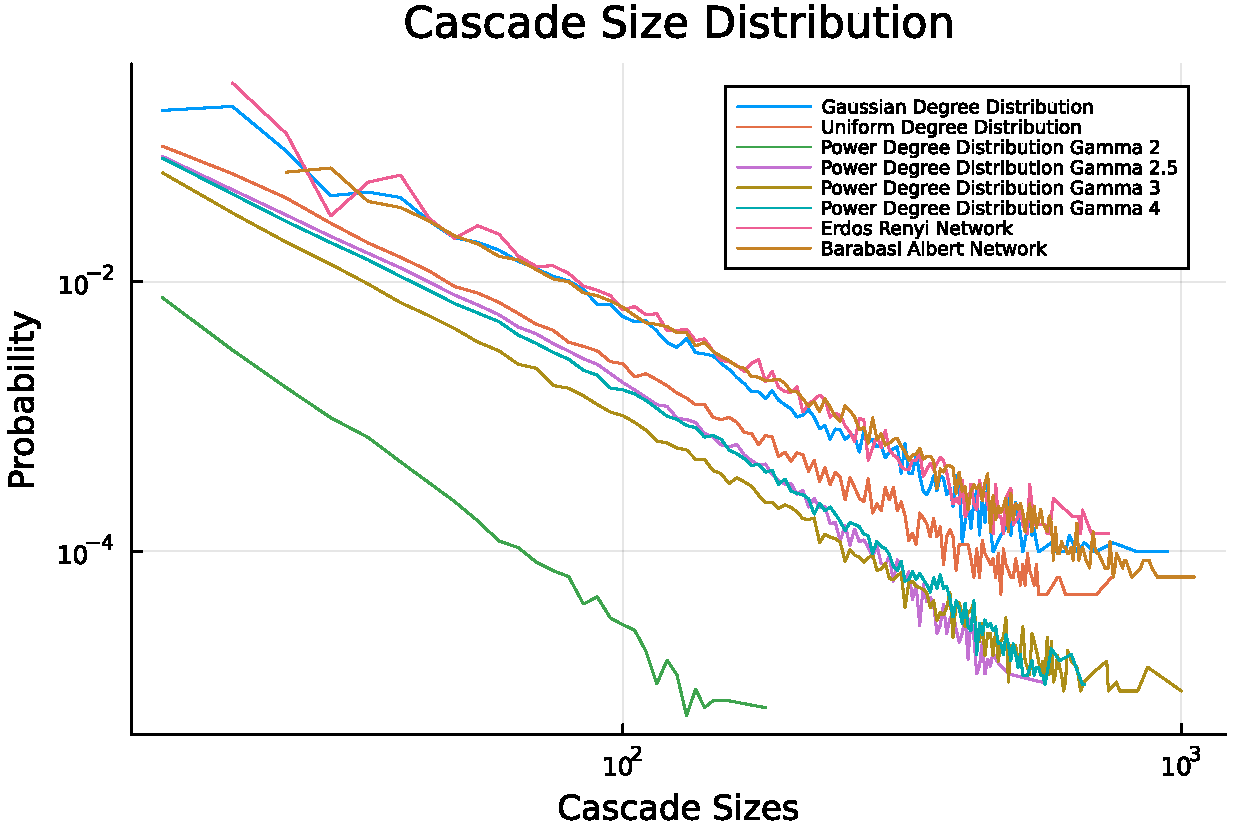
\includegraphics[width=0.5\textwidth]{images/Task15/AllNetworks.pdf}
        \caption{All Networks Size Distributions}
    \end{figure}

    
\newpage